\chapter{Optical Nonlinearity}

\section{Linear and nonlinear absorption}

Figure \ref{fig:linnonlinabsPP} show the \textit{Transmitted and Input power} of a 
linear and nonlinear absorber.

\begin{figure}[h!]
    \centering
    \includegraphics[width=0.75\textwidth]{slike/OptNonLin.pdf}
    \caption{Linear and nonlinear power absorption}
    \label{fig:linnonlinabsPP}
\end{figure}

In the linear absorber, absorption follows the \textit{Lambert-Beer's-Law} \pd $\frac{dI}{dx} = \alpha = const$. With 
the nonlinear absorber \pd $\frac{dI}{dx} = \alpha(I) \ne const $. With a high enough intensity all materials can become 
nonlinear. Nonlinearity has some application, such as SESAM, Laser structuring below with resolution lower than $\lambda$ \dots

\section{Origin of refractive index}
The refractive index originates from the interaction between
light (electromagnetic waves) and atoms. The electric filed forces the
atoms to oscillate, these oscillations are undamped with a frequency far 
from the atom's resonance frequency. 
Driving force of the oscillations synchronous to filed amplitude of
plane wave at the beginning. \textit{Strength} and \textit{phase} of oscilations 
depend on:
\begin{itemize}
    \item Electron/atom mass
    \item Charge distribution (electron orbital)
    \item Number of atoms
    \item Excitation frequency (Driving frequency)
    \item Difference between excitation and resonance frequency
\end{itemize}

Oscillating electrons create additional propagating EM waves at the same frequency 
but with a \textit{phase shift}. New waves \textbf{superimpose} with the original (excitation) wave and 
alter its propagation. They form new wave with a modified phase.

When the original wave moves deeper into the material, each atomic layer induces new EM waves, 
which generate more waves. All of these waves superimpose and modify the phase of the 
overall wave. 

The \textbf{macroscopic refractive index} results from the combined phase shift 
of the combined waves. 
The \textit{macro} refractive index depends on the atomic charge distribution, wavelength/frequency of the light and interaction 
of induced EM waves. Change of speed in the material depends on the strength of the field in material. 

In some cases, the refractive index can be less than $1$, meaning the \textbf{phase} velocity of light in the material 
can exceed the speed of light in vacuum, but the leading edge has already traveled through the material.


The motion of electron means that the energy of the initial EM wave 
is just temporarily stored  be the electron motion as a kind of $potential \, kinetic + electostatci \, energy$,
which is given off as a new EM wave later on \pd a \textbf{Perfectly transparent material can exist}, not a 
single molecule gets excited to a higher level.

\subsection{Influence of atomic structure on refractive index}

Refractive index depends on how electrons interact with an external electric filed. 
Electromagnetic wave consists of oscillating electric and magnetic fields, 
the electric field exerts a force on electrons in an atom, causing them to shift from their equilibrium position.
Electrons then experience a restoring force due to the attraction in the core. In an AC field
electrons oscillate around their equilibrium, behaving like harmonic oscillators.

Behavior of electrons depends on the force in electric filed. Interaction with \textit{weak} wave forces the electrons in the mateial 
to oscillate  with the \textit{same frequency} and the \textit{polarization} remains the same as the original input wave. 
Resulting refractive index depends on the superposition of the waves. For \textit{weak} waves this system behaves \textbf{linearly}, the refractive index 
is constant and does not depend on the intensity of the light. 


When the incoming wave is \textbf{strong} the electron's motion is no longer a simple 
harmonic oscillation \pd the restoring force from the atom's core is no longer proportional 
to the displacement. Potential energy curve is no longer a parabola, show on figure \ref{fig:EMWsw}, and the
resulting wave is no longer sinusoidal, it contains additional components. The resulting 
EM wave is non-harmonic and new frequencies are generated \pd non-linear optical effects. 
With the increase of frequency, refractive index will change (\textit{Kerr effect}).


\begin{figure}[h!]
    \centering
    \includegraphics[width=0.45\textwidth]{slike/EMwIO.pdf}
    \caption{Input and output wave with non-parabolic path and effect}
    \label{fig:EMWsw}
\end{figure}

\subsection{Second harmonic generation}

Electric oscillations induced by a strong EM wave  results in outgoing EM wave to \textbf{no longer be } harmonic - they are \textit{anharmonic}.
Anharmonic oscillations are nonlinear due to the shape of potential, the nonlinearity of "spring constant"
becomes apparent. An additional EM-wave with double frequency will appear on top of the original one. 
Figure \ref{fig:secharm} shows the second harmonic.

\begin{figure}[h!]
    \centering
    \includegraphics[width=0.5\textwidth]{slike/secharm.pdf}
    \caption{Secondary harmonic}
    \label{fig:secharm}
\end{figure}

Only some materials/crystals are capable of producing second harmonics.

Mathematical formulation of nonlinear effects:
\begin{equation}
    \vec{\nabla}^2 \vec{E} = \varepsilon_0 \mu_0 \frac{\partial \vec{E}^2}{\partial t^2}  + \mu_0 \frac{\partial \vec{P}^2}{\partial t^2}
\end{equation}


\section{Applications of nonlinearity}

Some applications of nonlinearity that were already explained:
\begin{itemize}
    \item Kerr-effect and mode locking
    \item SESAM mode locking
    \item Laser structuring bellow resolution limit
    \item Lithography
    \item Additive manufacturing
\end{itemize}


\subsection{Second harmonic generation}

Second and third harmonic generation enable us to produce different wave lentgth $\lambda$ without using
different laser active materials - different $\lambda$ are much easier to achieve.

Figure \ref{fig:shgapp1} shows a simple laser wavelength generation. 
\begin{figure}[h!]
    \centering
    \includegraphics[width=0.5\textwidth]{slike/Shgapp1.pdf}
    \caption{Secondary harmonic - generation of new $\lambda$}
    \label{fig:shgapp1}
\end{figure}

Applications of this process are welding of copper with $\lambda = 512 nm$ with $1064nm$ base laser, generation of UV wavelengths and USP pulse duration measurments.

\subsubsection{Three wave mixing}
Three wave mixing is a generation of a \textit{new} third wave is generated from interactions with 
different and frequencies and directions.
Process: 
\begin{enumerate}
    \item A pump beam at $515 nm$ interacts nonlinearly with a signal beam at $1030 nm$.
    \item The $515 nm$ photon is stimulated by the $1030 nm$ photon to decay into two new photons at $1030 nm$.
\end{enumerate}

The process described is an example of optical parametric amplification (OPA),
where energy is transferred from the pump beam to the signal beam, 
resulting in an amplified signal and the generation of an entangled idler beam.

This is a very efficient way to amplify light without generating heat. 

We can also use an \textit{optical parametric oscillator} to create more photons of different $\lambda$. 
If a wave with $532 nm$ nonlinearly intreracts with photon of $1064 nm$, it ( photon with $532nm$) can split into two 
photons with $1064nm$. This amplifies the original $1064nm$ beam of light. 

Three wave mixing still \textit{respects} energy and momentum conservation \pd we are not creating new energy. 
Phase velocity between the original and new EM wave must be the same. 

\subsection{Third harmonic generation}
Third Harmonic Generation (THG) is achieved by using two sequential Three-Wave Mixing  stages in a nonlinear medium.
The first stage performs Second Harmonic Generation (SHG), doubling the frequency of the original wave, and the second
stage then mixes the SHG output with the original wave, creating a new wave with three times the original frequency (THG).
Direct THG is possible but has low efficiency, so the two-step process is preferred for practical applications. 
This method is useful for generating ultraviolet (UV) light and other high-frequency laser sources.

Figure \ref{fig:thg} shows the generation of the third harmonic.
\begin{figure}[h!]
    \centering
    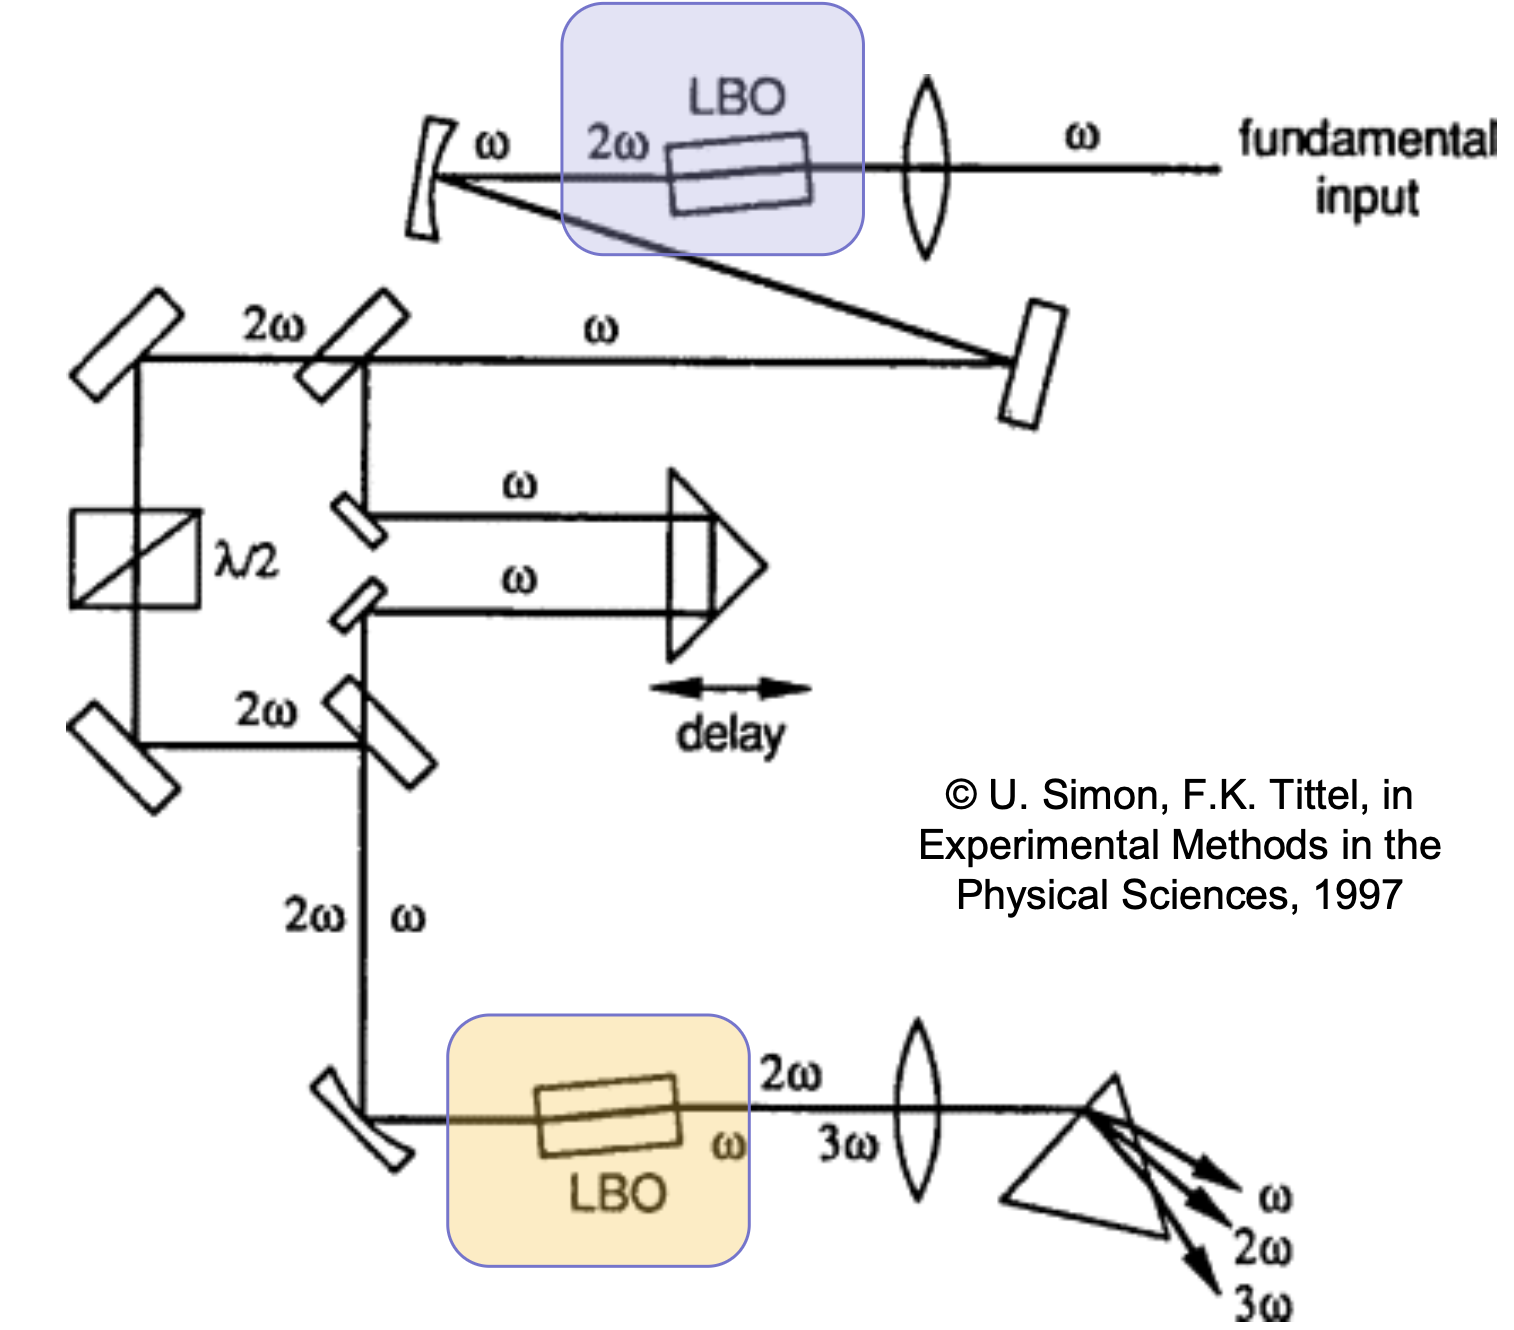
\includegraphics[width=0.5\textwidth]{slike/thg.png}
    \caption{Third harmonic generation }
    \label{fig:thg}
\end{figure}

\subsubsection{Applications of Third harmonic generation}
\begin{itemize}
    \item Due to THG UV wave length can be produces by solid state lasers. Coherence of UV light is almost the same 
            s of the initial laser source.
    \item Generation of ultrashort pulses and ultra powerful laser pulses. 
    \item Tunable, coherent radiation on the spectrum of UV to THz
    \item Important for quantum optics
\end{itemize}

\subsection{Ultra-short pulse duration measurements}
USP pulses last from \textit{attosecond to picosecond } \pd $10^{-18} to 10^{-12}$s. 
No electronics are fast enough to measure such short durations.

Technique called \textbf{nonlinear autocorrelation} is used to measure the pulse duration. 
A laser pulse is split into two pulses that travel a path different length, which causes a delay. The delay is controlled with a movable mirror.
Pulses are then recombined in a nonlinear crystal, where they interact only when they overlap in time. Because the autocorrelation only
occurs when both pulses are present its signal provides the information about pulse duration. 
The experimental setup includes a beam splitter, a delay line, a nonlinear crystal  and a detector.

\subsection{Chirped pulse amplification}


Chirped pulse amplification (CPA), shown on figure \ref{fig:cpa}, is a process in which we stretch the pulse in time, using a dispersive medium, 
and amplify it without damaging the components. After amplification, we again shorten the pulse back to its 
original duration, this results in a very intense and very short pulse. 

\begin{figure}[h!]
    \centering
    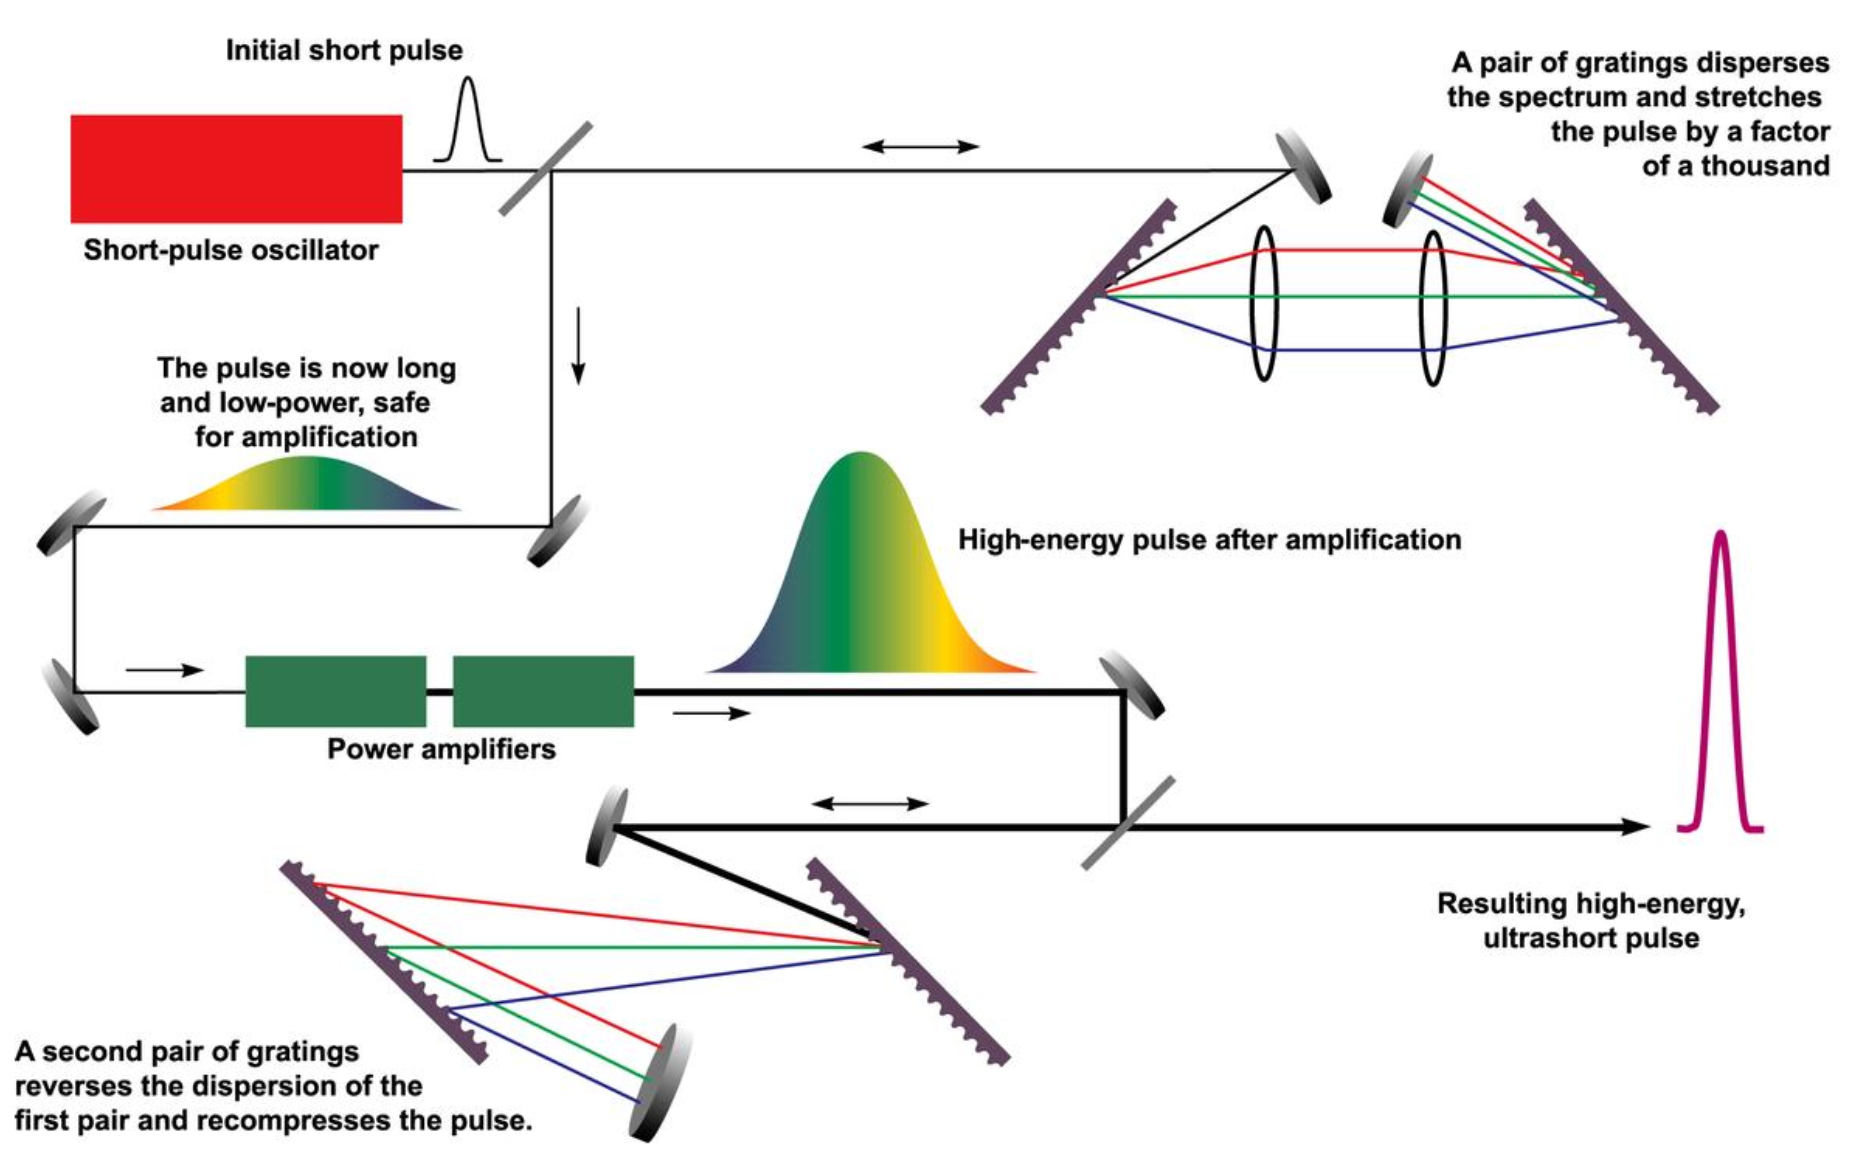
\includegraphics[width=0.75\textwidth]{slike/cpa.png}
    \caption{CPA}
    \label{fig:cpa}
\end{figure}

\section*{}